\documentclass[1p]{elsarticle_modified}
%\bibliographystyle{elsarticle-num}

%\usepackage[colorlinks]{hyperref}
%\usepackage{abbrmath_seonhwa} %\Abb, \Ascr, \Acal ,\Abf, \Afrak
\usepackage{amsfonts}
\usepackage{amssymb}
\usepackage{amsmath}
\usepackage{amsthm}
\usepackage{scalefnt}
\usepackage{amsbsy}
\usepackage{kotex}
\usepackage{caption}
\usepackage{subfig}
\usepackage{color}
\usepackage{graphicx}
\usepackage{xcolor} %% white, black, red, green, blue, cyan, magenta, yellow
\usepackage{float}
\usepackage{setspace}
\usepackage{hyperref}

\usepackage{tikz}
\usetikzlibrary{arrows}

\usepackage{multirow}
\usepackage{array} % fixed length table
\usepackage{hhline}

%%%%%%%%%%%%%%%%%%%%%
\makeatletter
\renewcommand*\env@matrix[1][\arraystretch]{%
	\edef\arraystretch{#1}%
	\hskip -\arraycolsep
	\let\@ifnextchar\new@ifnextchar
	\array{*\c@MaxMatrixCols c}}
\makeatother %https://tex.stackexchange.com/questions/14071/how-can-i-increase-the-line-spacing-in-a-matrix
%%%%%%%%%%%%%%%

\usepackage[normalem]{ulem}

\newcommand{\msout}[1]{\ifmmode\text{\sout{\ensuremath{#1}}}\else\sout{#1}\fi}
%SOURCE: \msout is \stkout macro in https://tex.stackexchange.com/questions/20609/strikeout-in-math-mode

\newcommand{\cancel}[1]{
	\ifmmode
	{\color{red}\msout{#1}}
	\else
	{\color{red}\sout{#1}}
	\fi
}

\newcommand{\add}[1]{
	{\color{blue}\uwave{#1}}
}

\newcommand{\replace}[2]{
	\ifmmode
	{\color{red}\msout{#1}}{\color{blue}\uwave{#2}}
	\else
	{\color{red}\sout{#1}}{\color{blue}\uwave{#2}}
	\fi
}

\newcommand{\Sol}{\mathcal{S}} %segment
\newcommand{\D}{D} %diagram
\newcommand{\A}{\mathcal{A}} %arc


%%%%%%%%%%%%%%%%%%%%%%%%%%%%%5 test

\def\sl{\operatorname{\textup{SL}}(2,\Cbb)}
\def\psl{\operatorname{\textup{PSL}}(2,\Cbb)}
\def\quan{\mkern 1mu \triangleright \mkern 1mu}

\theoremstyle{definition}
\newtheorem{thm}{Theorem}[section]
\newtheorem{prop}[thm]{Proposition}
\newtheorem{lem}[thm]{Lemma}
\newtheorem{ques}[thm]{Question}
\newtheorem{cor}[thm]{Corollary}
\newtheorem{defn}[thm]{Definition}
\newtheorem{exam}[thm]{Example}
\newtheorem{rmk}[thm]{Remark}
\newtheorem{alg}[thm]{Algorithm}

\newcommand{\I}{\sqrt{-1}}
\begin{document}

%\begin{frontmatter}
%
%\title{Boundary parabolic representations of knots up to 8 crossings}
%
%%% Group authors per affiliation:
%\author{Yunhi Cho} 
%\address{Department of Mathematics, University of Seoul, Seoul, Korea}
%\ead{yhcho@uos.ac.kr}
%
%
%\author{Seonhwa Kim} %\fnref{s_kim}}
%\address{Center for Geometry and Physics, Institute for Basic Science, Pohang, 37673, Korea}
%\ead{ryeona17@ibs.re.kr}
%
%\author{Hyuk Kim}
%\address{Department of Mathematical Sciences, Seoul National University, Seoul 08826, Korea}
%\ead{hyukkim@snu.ac.kr}
%
%\author{Seokbeom Yoon}
%\address{Department of Mathematical Sciences, Seoul National University, Seoul, 08826,  Korea}
%\ead{sbyoon15@snu.ac.kr}
%
%\begin{abstract}
%We find all boundary parabolic representation of knots up to 8 crossings.
%
%\end{abstract}
%\begin{keyword}
%    \MSC[2010] 57M25 
%\end{keyword}
%
%\end{frontmatter}

%\linenumbers
%\tableofcontents
%
\newcommand\colored[1]{\textcolor{white}{\rule[-0.35ex]{0.8em}{1.4ex}}\kern-0.8em\color{red} #1}%
%\newcommand\colored[1]{\textcolor{white}{ #1}\kern-2.17ex	\textcolor{white}{ #1}\kern-1.81ex	\textcolor{white}{ #1}\kern-2.15ex\color{red}#1	}

{\Large $\underline{12a_{0678}~(K12a_{0678})}$}

\setlength{\tabcolsep}{10pt}
\renewcommand{\arraystretch}{1.6}
\vspace{1cm}\begin{tabular}{m{100pt}>{\centering\arraybackslash}m{274pt}}
\multirow{5}{120pt}{
	\centering
	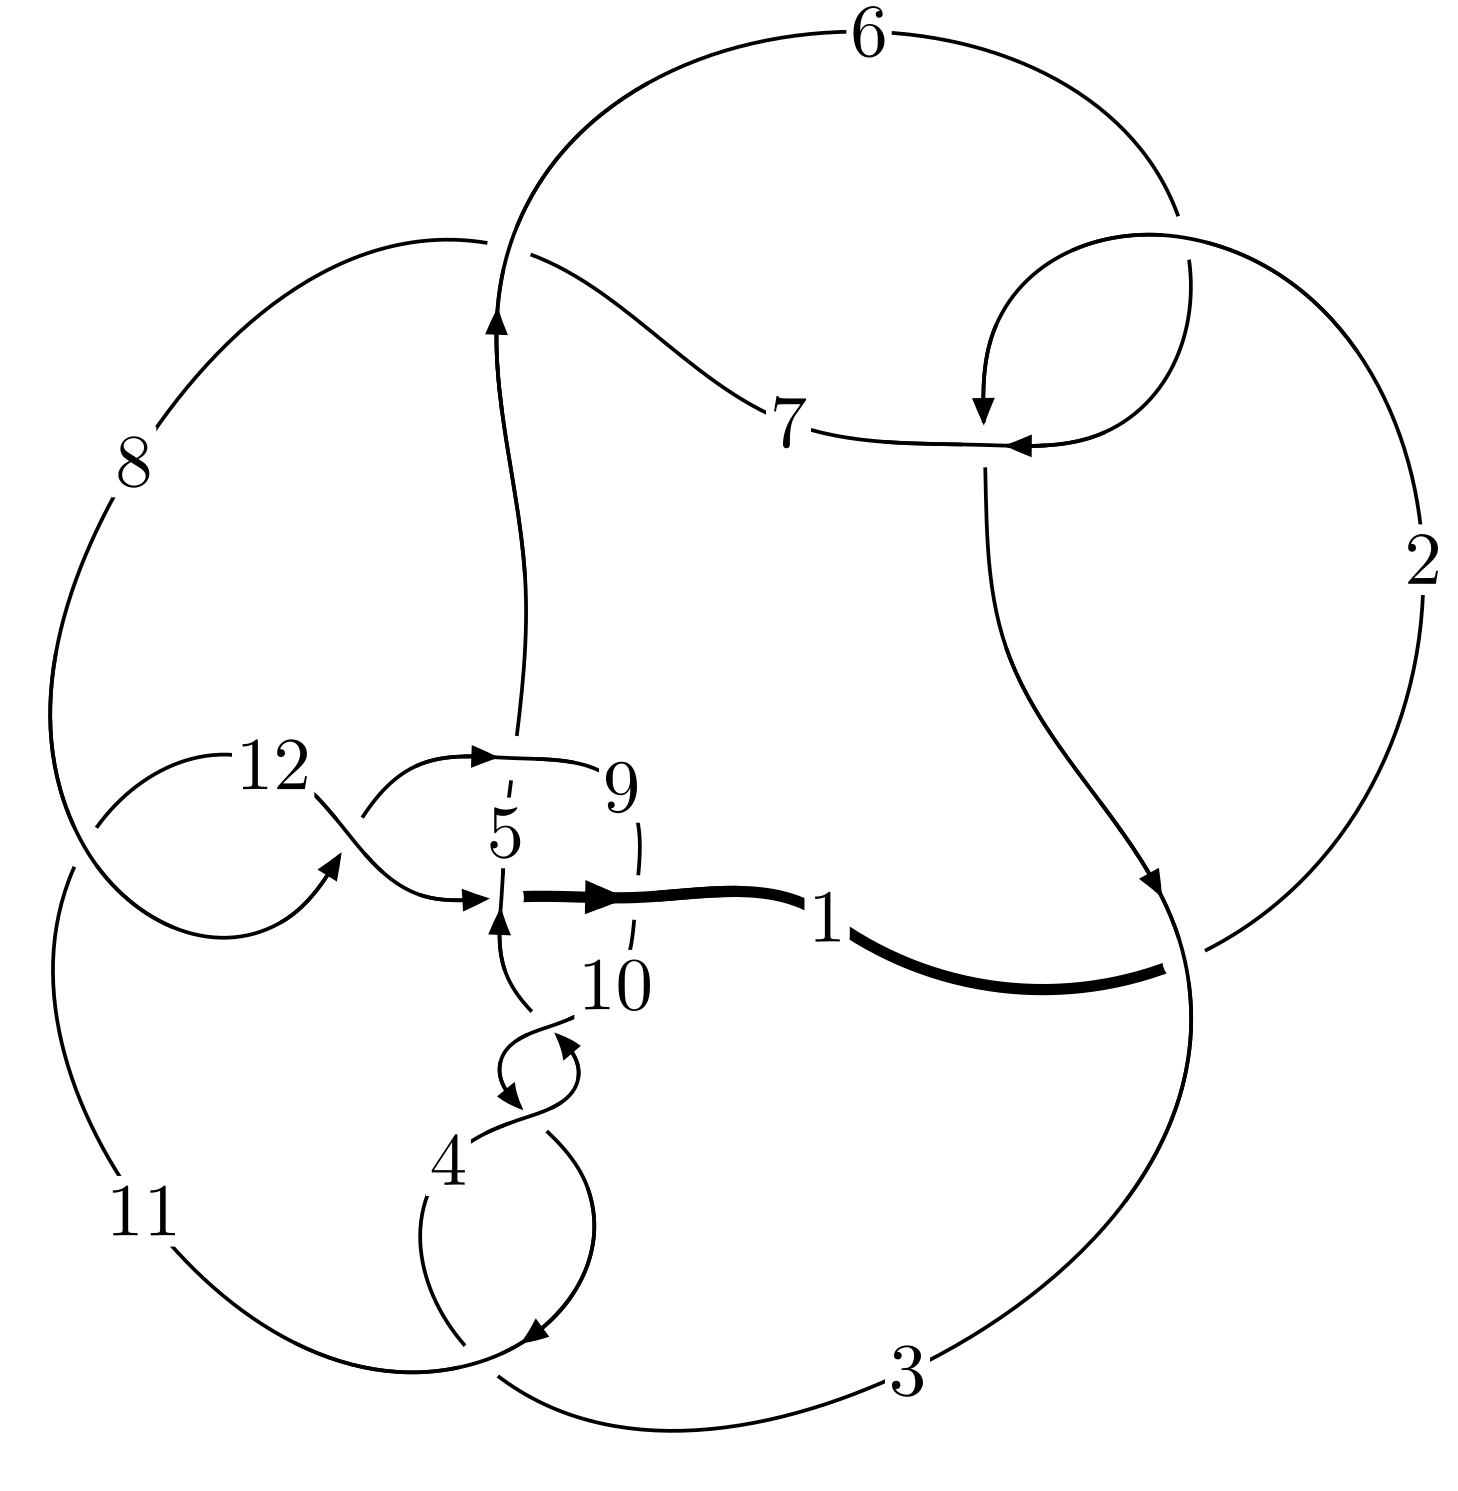
\includegraphics[width=112pt]{../../../GIT/diagram.site/Diagrams/png/1479_12a_0678.png}\\
\ \ \ A knot diagram\footnotemark}&
\allowdisplaybreaks
\textbf{Linearized knot diagam} \\
\cline{2-2}
 &
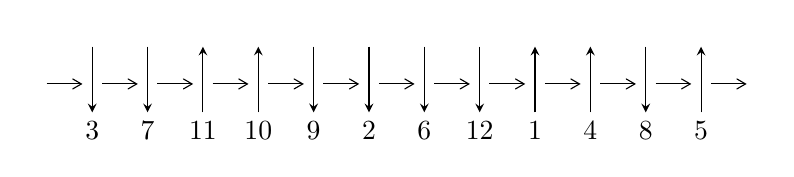
\begin{tikzpicture}[x=20pt, y=17pt]
	% nodes
	\node (C0) at (0, 0) {};
	\node (C1) at (1, 0) {};
	\node (C1U) at (1, +1) {};
	\node (C1D) at (1, -1) {3};

	\node (C2) at (2, 0) {};
	\node (C2U) at (2, +1) {};
	\node (C2D) at (2, -1) {7};

	\node (C3) at (3, 0) {};
	\node (C3U) at (3, +1) {};
	\node (C3D) at (3, -1) {11};

	\node (C4) at (4, 0) {};
	\node (C4U) at (4, +1) {};
	\node (C4D) at (4, -1) {10};

	\node (C5) at (5, 0) {};
	\node (C5U) at (5, +1) {};
	\node (C5D) at (5, -1) {9};

	\node (C6) at (6, 0) {};
	\node (C6U) at (6, +1) {};
	\node (C6D) at (6, -1) {2};

	\node (C7) at (7, 0) {};
	\node (C7U) at (7, +1) {};
	\node (C7D) at (7, -1) {6};

	\node (C8) at (8, 0) {};
	\node (C8U) at (8, +1) {};
	\node (C8D) at (8, -1) {12};

	\node (C9) at (9, 0) {};
	\node (C9U) at (9, +1) {};
	\node (C9D) at (9, -1) {1};

	\node (C10) at (10, 0) {};
	\node (C10U) at (10, +1) {};
	\node (C10D) at (10, -1) {4};

	\node (C11) at (11, 0) {};
	\node (C11U) at (11, +1) {};
	\node (C11D) at (11, -1) {8};

	\node (C12) at (12, 0) {};
	\node (C12U) at (12, +1) {};
	\node (C12D) at (12, -1) {5};
	\node (C13) at (13, 0) {};

	% arrows
	\draw[->,>={angle 60}]
	(C0) edge (C1) (C1) edge (C2) (C2) edge (C3) (C3) edge (C4) (C4) edge (C5) (C5) edge (C6) (C6) edge (C7) (C7) edge (C8) (C8) edge (C9) (C9) edge (C10) (C10) edge (C11) (C11) edge (C12) (C12) edge (C13) ;	\draw[->,>=stealth]
	(C1U) edge (C1D) (C2U) edge (C2D) (C3D) edge (C3U) (C4D) edge (C4U) (C5U) edge (C5D) (C6U) edge (C6D) (C7U) edge (C7D) (C8U) edge (C8D) (C9D) edge (C9U) (C10D) edge (C10U) (C11U) edge (C11D) (C12D) edge (C12U) ;
	\end{tikzpicture} \\
\hhline{~~} \\& 
\textbf{Solving Sequence} \\ \cline{2-2} 
 &
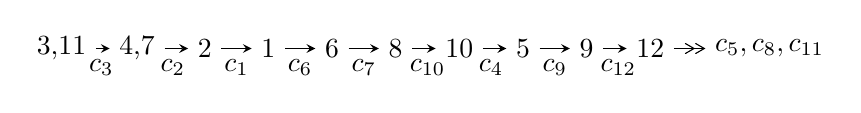
\begin{tikzpicture}[x=23pt, y=7pt]
	% node
	\node (A0) at (-1/8, 0) {3,11};
	\node (A1) at (17/16, 0) {4,7};
	\node (A2) at (17/8, 0) {2};
	\node (A3) at (25/8, 0) {1};
	\node (A4) at (33/8, 0) {6};
	\node (A5) at (41/8, 0) {8};
	\node (A6) at (49/8, 0) {10};
	\node (A7) at (57/8, 0) {5};
	\node (A8) at (65/8, 0) {9};
	\node (A9) at (73/8, 0) {12};
	\node (C1) at (1/2, -1) {$c_{3}$};
	\node (C2) at (13/8, -1) {$c_{2}$};
	\node (C3) at (21/8, -1) {$c_{1}$};
	\node (C4) at (29/8, -1) {$c_{6}$};
	\node (C5) at (37/8, -1) {$c_{7}$};
	\node (C6) at (45/8, -1) {$c_{10}$};
	\node (C7) at (53/8, -1) {$c_{4}$};
	\node (C8) at (61/8, -1) {$c_{9}$};
	\node (C9) at (69/8, -1) {$c_{12}$};
	\node (A10) at (11, 0) {$c_{5},c_{8},c_{11}$};

	% edge
	\draw[->,>=stealth]	
	(A0) edge (A1) (A1) edge (A2) (A2) edge (A3) (A3) edge (A4) (A4) edge (A5) (A5) edge (A6) (A6) edge (A7) (A7) edge (A8) (A8) edge (A9) ;
	\draw[->>,>={angle 60}]	
	(A9) edge (A10);
\end{tikzpicture} \\ 

\end{tabular} \\

\footnotetext{
The image of knot diagram is generated by the software ``\textbf{Draw programme}" developed by Andrew Bartholomew(\url{http://www.layer8.co.uk/maths/draw/index.htm\#Running-draw}), where we modified some parts for our purpose(\url{https://github.com/CATsTAILs/LinksPainter}).
}\phantom \\ \newline 
\centering \textbf{Ideals for irreducible components\footnotemark of $X_{\text{par}}$} 
 
\begin{align*}
I^u_{1}&=\langle 
2.88041\times10^{309} u^{112}+8.48809\times10^{308} u^{111}+\cdots+1.65652\times10^{311} b-2.44967\times10^{311},\\
\phantom{I^u_{1}}&\phantom{= \langle  }3.34457\times10^{311} u^{112}-3.90481\times10^{311} u^{111}+\cdots+1.82217\times10^{312} a+1.06215\times10^{313},\\
\phantom{I^u_{1}}&\phantom{= \langle  }u^{113}- u^{112}+\cdots+15 u+11\rangle \\
I^u_{2}&=\langle 
3 u^{22}+38 u^{20}+\cdots+b+2,\;u^{19}+11 u^{17}+\cdots+a+1,\;u^{24}+14 u^{22}+\cdots+2 u+1\rangle \\
\\
\end{align*}
\raggedright * 2 irreducible components of $\dim_{\mathbb{C}}=0$, with total 137 representations.\\
\footnotetext{All coefficients of polynomials are rational numbers. But the coefficients are sometimes approximated in decimal forms when there is not enough margin.}
\newpage
\renewcommand{\arraystretch}{1}
\centering \section*{I. $I^u_{1}= \langle 2.88\times10^{309} u^{112}+8.49\times10^{308} u^{111}+\cdots+1.66\times10^{311} b-2.45\times10^{311},\;3.34\times10^{311} u^{112}-3.90\times10^{311} u^{111}+\cdots+1.82\times10^{312} a+1.06\times10^{313},\;u^{113}- u^{112}+\cdots+15 u+11 \rangle$}
\flushleft \textbf{(i) Arc colorings}\\
\begin{tabular}{m{7pt} m{180pt} m{7pt} m{180pt} }
\flushright $a_{3}=$&$\begin{pmatrix}1\\0\end{pmatrix}$ \\
\flushright $a_{11}=$&$\begin{pmatrix}0\\u\end{pmatrix}$ \\
\flushright $a_{4}=$&$\begin{pmatrix}1\\- u^2\end{pmatrix}$ \\
\flushright $a_{7}=$&$\begin{pmatrix}-0.183549 u^{112}+0.214295 u^{111}+\cdots-20.6174 u-5.82903\\-0.0173884 u^{112}-0.00512406 u^{111}+\cdots-0.0536761 u+1.47881\end{pmatrix}$ \\
\flushright $a_{2}=$&$\begin{pmatrix}0.132513 u^{112}-0.169681 u^{111}+\cdots+8.54221 u+0.737478\\-0.0162259 u^{112}-0.0501027 u^{111}+\cdots-1.92847 u-0.675743\end{pmatrix}$ \\
\flushright $a_{1}=$&$\begin{pmatrix}0.116287 u^{112}-0.219784 u^{111}+\cdots+6.61374 u+0.0617348\\-0.0162259 u^{112}-0.0501027 u^{111}+\cdots-1.92847 u-0.675743\end{pmatrix}$ \\
\flushright $a_{6}=$&$\begin{pmatrix}-0.0974973 u^{112}+0.157066 u^{111}+\cdots-25.6173 u-11.7732\\-0.00678329 u^{112}-0.0287232 u^{111}+\cdots+1.40250 u+2.02414\end{pmatrix}$ \\
\flushright $a_{8}=$&$\begin{pmatrix}0.154016 u^{112}-0.165009 u^{111}+\cdots-12.0342 u+0.764893\\0.0218718 u^{112}-0.0968420 u^{111}+\cdots+2.52686 u-1.37446\end{pmatrix}$ \\
\flushright $a_{10}=$&$\begin{pmatrix}- u\\u^3+u\end{pmatrix}$ \\
\flushright $a_{5}=$&$\begin{pmatrix}u^2+1\\- u^4-2 u^2\end{pmatrix}$ \\
\flushright $a_{9}=$&$\begin{pmatrix}-0.129130 u^{112}+0.113392 u^{111}+\cdots+59.8830 u-2.07616\\-0.0181661 u^{112}+0.0738493 u^{111}+\cdots-7.90164 u+1.00539\end{pmatrix}$ \\
\flushright $a_{12}=$&$\begin{pmatrix}0.125690 u^{112}-0.165723 u^{111}+\cdots+10.2798 u+0.288716\\-0.00525691 u^{112}-0.0914473 u^{111}+\cdots-1.96487 u-1.01948\end{pmatrix}$\\&\end{tabular}
\flushleft \textbf{(ii) Obstruction class $= -1$}\\~\\
\flushleft \textbf{(iii) Cusp Shapes $= 0.101122 u^{112}-0.0898832 u^{111}+\cdots+12.7383 u-7.53310$}\\~\\
\newpage\renewcommand{\arraystretch}{1}
\flushleft \textbf{(iv) u-Polynomials at the component}\newline \\
\begin{tabular}{m{50pt}|m{274pt}}
Crossings & \hspace{64pt}u-Polynomials at each crossing \\
\hline $$\begin{aligned}c_{1},c_{7}\end{aligned}$$&$\begin{aligned}
&u^{113}+39 u^{112}+\cdots-216 u+1
\end{aligned}$\\
\hline $$\begin{aligned}c_{2},c_{6}\end{aligned}$$&$\begin{aligned}
&u^{113}- u^{112}+\cdots+12 u+1
\end{aligned}$\\
\hline $$\begin{aligned}c_{3},c_{4},c_{10}\end{aligned}$$&$\begin{aligned}
&u^{113}- u^{112}+\cdots+15 u+11
\end{aligned}$\\
\hline $$\begin{aligned}c_{5}\end{aligned}$$&$\begin{aligned}
&u^{113}-5 u^{112}+\cdots+240 u-13
\end{aligned}$\\
\hline $$\begin{aligned}c_{8},c_{11}\end{aligned}$$&$\begin{aligned}
&u^{113}- u^{112}+\cdots-2039 u-229
\end{aligned}$\\
\hline $$\begin{aligned}c_{9}\end{aligned}$$&$\begin{aligned}
&u^{113}-7 u^{112}+\cdots-7067 u-2507
\end{aligned}$\\
\hline $$\begin{aligned}c_{12}\end{aligned}$$&$\begin{aligned}
&u^{113}-4 u^{112}+\cdots+56403 u+23683
\end{aligned}$\\
\hline
\end{tabular}\\~\\
\newpage\renewcommand{\arraystretch}{1}
\flushleft \textbf{(v) Riley Polynomials at the component}\newline \\
\begin{tabular}{m{50pt}|m{274pt}}
Crossings & \hspace{64pt}Riley Polynomials at each crossing \\
\hline $$\begin{aligned}c_{1},c_{7}\end{aligned}$$&$\begin{aligned}
&y^{113}+81 y^{112}+\cdots-11600 y-1
\end{aligned}$\\
\hline $$\begin{aligned}c_{2},c_{6}\end{aligned}$$&$\begin{aligned}
&y^{113}-39 y^{112}+\cdots-216 y-1
\end{aligned}$\\
\hline $$\begin{aligned}c_{3},c_{4},c_{10}\end{aligned}$$&$\begin{aligned}
&y^{113}+115 y^{112}+\cdots+5989 y-121
\end{aligned}$\\
\hline $$\begin{aligned}c_{5}\end{aligned}$$&$\begin{aligned}
&y^{113}-7 y^{112}+\cdots-4228 y-169
\end{aligned}$\\
\hline $$\begin{aligned}c_{8},c_{11}\end{aligned}$$&$\begin{aligned}
&y^{113}-81 y^{112}+\cdots-193937 y-52441
\end{aligned}$\\
\hline $$\begin{aligned}c_{9}\end{aligned}$$&$\begin{aligned}
&y^{113}+17 y^{112}+\cdots-196420401 y-6285049
\end{aligned}$\\
\hline $$\begin{aligned}c_{12}\end{aligned}$$&$\begin{aligned}
&y^{113}+40 y^{112}+\cdots-26878017779 y-560884489
\end{aligned}$\\
\hline
\end{tabular}\\~\\
\newpage\flushleft \textbf{(vi) Complex Volumes and Cusp Shapes}
$$\begin{array}{c|c|c}  
\text{Solutions to }I^u_{1}& \I (\text{vol} + \sqrt{-1}CS) & \text{Cusp shape}\\
 \hline 
\begin{aligned}
u &= -0.904745 + 0.460220 I \\
a &= -0.96192 + 1.22457 I \\
b &= \phantom{-}0.688613 - 0.837945 I\end{aligned}
 & \phantom{-}1.45825 - 7.28472 I & \phantom{-0.000000 } 0 \\ \hline\begin{aligned}
u &= -0.904745 - 0.460220 I \\
a &= -0.96192 - 1.22457 I \\
b &= \phantom{-}0.688613 + 0.837945 I\end{aligned}
 & \phantom{-}1.45825 + 7.28472 I & \phantom{-0.000000 } 0 \\ \hline\begin{aligned}
u &= -0.296641 + 0.935465 I \\
a &= -0.044155 + 0.326319 I \\
b &= \phantom{-}0.936373 - 0.712759 I\end{aligned}
 & -0.50638 + 3.02045 I & \phantom{-0.000000 } 0 \\ \hline\begin{aligned}
u &= -0.296641 - 0.935465 I \\
a &= -0.044155 - 0.326319 I \\
b &= \phantom{-}0.936373 + 0.712759 I\end{aligned}
 & -0.50638 - 3.02045 I & \phantom{-0.000000 } 0 \\ \hline\begin{aligned}
u &= \phantom{-}1.017070 + 0.148681 I \\
a &= \phantom{-}0.88000 - 1.91335 I \\
b &= -0.948912 + 0.670284 I\end{aligned}
 & -0.82794 + 3.11768 I & \phantom{-0.000000 } 0 \\ \hline\begin{aligned}
u &= \phantom{-}1.017070 - 0.148681 I \\
a &= \phantom{-}0.88000 + 1.91335 I \\
b &= -0.948912 - 0.670284 I\end{aligned}
 & -0.82794 - 3.11768 I & \phantom{-0.000000 } 0 \\ \hline\begin{aligned}
u &= \phantom{-}0.717168 + 0.646184 I \\
a &= -0.113524 - 0.620470 I \\
b &= -1.064940 + 0.175863 I\end{aligned}
 & -5.34748 + 7.31945 I & \phantom{-0.000000 } 0 \\ \hline\begin{aligned}
u &= \phantom{-}0.717168 - 0.646184 I \\
a &= -0.113524 + 0.620470 I \\
b &= -1.064940 - 0.175863 I\end{aligned}
 & -5.34748 - 7.31945 I & \phantom{-0.000000 } 0 \\ \hline\begin{aligned}
u &= \phantom{-}0.961035 + 0.501171 I \\
a &= -0.130517 + 0.522604 I \\
b &= \phantom{-}0.966771 + 0.026860 I\end{aligned}
 & -4.61135 - 1.81073 I & \phantom{-0.000000 } 0 \\ \hline\begin{aligned}
u &= \phantom{-}0.961035 - 0.501171 I \\
a &= -0.130517 - 0.522604 I \\
b &= \phantom{-}0.966771 - 0.026860 I\end{aligned}
 & -4.61135 + 1.81073 I & \phantom{-0.000000 } 0\\
 \hline 
 \end{array}$$\newpage$$\begin{array}{c|c|c}  
\text{Solutions to }I^u_{1}& \I (\text{vol} + \sqrt{-1}CS) & \text{Cusp shape}\\
 \hline 
\begin{aligned}
u &= \phantom{-}0.952030 + 0.520069 I \\
a &= -0.15869 + 1.98165 I \\
b &= \phantom{-}1.021830 - 0.732336 I\end{aligned}
 & \phantom{-}0.43907 + 13.15560 I & \phantom{-0.000000 } 0 \\ \hline\begin{aligned}
u &= \phantom{-}0.952030 - 0.520069 I \\
a &= -0.15869 - 1.98165 I \\
b &= \phantom{-}1.021830 + 0.732336 I\end{aligned}
 & \phantom{-}0.43907 - 13.15560 I & \phantom{-0.000000 } 0 \\ \hline\begin{aligned}
u &= -0.889860 + 0.051884 I \\
a &= \phantom{-}0.84685 - 2.15997 I \\
b &= -0.758557 + 0.674541 I\end{aligned}
 & -0.23754 + 2.10414 I & \phantom{-0.000000 } 0 \\ \hline\begin{aligned}
u &= -0.889860 - 0.051884 I \\
a &= \phantom{-}0.84685 + 2.15997 I \\
b &= -0.758557 - 0.674541 I\end{aligned}
 & -0.23754 - 2.10414 I & \phantom{-0.000000 } 0 \\ \hline\begin{aligned}
u &= \phantom{-}0.257866 + 1.091200 I \\
a &= \phantom{-}0.369039 + 1.068280 I \\
b &= \phantom{-}0.794720 - 0.766604 I\end{aligned}
 & -0.07099 + 2.58407 I & \phantom{-0.000000 } 0 \\ \hline\begin{aligned}
u &= \phantom{-}0.257866 - 1.091200 I \\
a &= \phantom{-}0.369039 - 1.068280 I \\
b &= \phantom{-}0.794720 + 0.766604 I\end{aligned}
 & -0.07099 - 2.58407 I & \phantom{-0.000000 } 0 \\ \hline\begin{aligned}
u &= \phantom{-}0.040879 + 0.851393 I \\
a &= \phantom{-}0.554820 + 0.537590 I \\
b &= \phantom{-}0.497920 - 0.402888 I\end{aligned}
 & -0.94803 + 1.45359 I & \phantom{-0.000000 } 0 \\ \hline\begin{aligned}
u &= \phantom{-}0.040879 - 0.851393 I \\
a &= \phantom{-}0.554820 - 0.537590 I \\
b &= \phantom{-}0.497920 + 0.402888 I\end{aligned}
 & -0.94803 - 1.45359 I & \phantom{-0.000000 } 0 \\ \hline\begin{aligned}
u &= -0.672021 + 0.499691 I \\
a &= \phantom{-}0.39256 - 2.25417 I \\
b &= \phantom{-}0.946144 + 0.752331 I\end{aligned}
 & \phantom{-}4.60985 - 7.30372 I & \phantom{-0.000000 } 0 \\ \hline\begin{aligned}
u &= -0.672021 - 0.499691 I \\
a &= \phantom{-}0.39256 + 2.25417 I \\
b &= \phantom{-}0.946144 - 0.752331 I\end{aligned}
 & \phantom{-}4.60985 + 7.30372 I & \phantom{-0.000000 } 0\\
 \hline 
 \end{array}$$\newpage$$\begin{array}{c|c|c}  
\text{Solutions to }I^u_{1}& \I (\text{vol} + \sqrt{-1}CS) & \text{Cusp shape}\\
 \hline 
\begin{aligned}
u &= \phantom{-}0.700086 + 0.431320 I \\
a &= -1.28265 - 0.73113 I \\
b &= \phantom{-}0.794688 + 0.790567 I\end{aligned}
 & \phantom{-}5.07217 + 1.49536 I & \phantom{-0.000000 } 0 \\ \hline\begin{aligned}
u &= \phantom{-}0.700086 - 0.431320 I \\
a &= -1.28265 + 0.73113 I \\
b &= \phantom{-}0.794688 - 0.790567 I\end{aligned}
 & \phantom{-}5.07217 - 1.49536 I & \phantom{-0.000000 } 0 \\ \hline\begin{aligned}
u &= -0.872118 + 0.855001 I \\
a &= \phantom{-}0.02346 + 1.69483 I \\
b &= -0.735758 - 0.728083 I\end{aligned}
 & \phantom{-}0.45892 + 1.35049 I & \phantom{-0.000000 } 0 \\ \hline\begin{aligned}
u &= -0.872118 - 0.855001 I \\
a &= \phantom{-}0.02346 - 1.69483 I \\
b &= -0.735758 + 0.728083 I\end{aligned}
 & \phantom{-}0.45892 - 1.35049 I & \phantom{-0.000000 } 0 \\ \hline\begin{aligned}
u &= \phantom{-}0.485816 + 0.594222 I \\
a &= -0.00749 - 1.74016 I \\
b &= -0.885101 + 0.783586 I\end{aligned}
 & \phantom{-}4.45524 + 2.73268 I & \phantom{-0.000000 } 0. - 3.15176 I \\ \hline\begin{aligned}
u &= \phantom{-}0.485816 - 0.594222 I \\
a &= -0.00749 + 1.74016 I \\
b &= -0.885101 - 0.783586 I\end{aligned}
 & \phantom{-}4.45524 - 2.73268 I & \phantom{-0.000000 -}0. + 3.15176 I \\ \hline\begin{aligned}
u &= -0.030242 + 1.257560 I \\
a &= \phantom{-}0.746401 + 0.445817 I \\
b &= -0.810158 + 0.596598 I\end{aligned}
 & -4.05059 + 5.07742 I & \phantom{-0.000000 } 0 \\ \hline\begin{aligned}
u &= -0.030242 - 1.257560 I \\
a &= \phantom{-}0.746401 - 0.445817 I \\
b &= -0.810158 - 0.596598 I\end{aligned}
 & -4.05059 - 5.07742 I & \phantom{-0.000000 } 0 \\ \hline\begin{aligned}
u &= \phantom{-}0.976987 + 0.815948 I \\
a &= \phantom{-}0.603989 + 1.014990 I \\
b &= -0.967712 - 0.693262 I\end{aligned}
 & -0.24807 - 6.79516 I & \phantom{-0.000000 } 0 \\ \hline\begin{aligned}
u &= \phantom{-}0.976987 - 0.815948 I \\
a &= \phantom{-}0.603989 - 1.014990 I \\
b &= -0.967712 + 0.693262 I\end{aligned}
 & -0.24807 + 6.79516 I & \phantom{-0.000000 } 0\\
 \hline 
 \end{array}$$\newpage$$\begin{array}{c|c|c}  
\text{Solutions to }I^u_{1}& \I (\text{vol} + \sqrt{-1}CS) & \text{Cusp shape}\\
 \hline 
\begin{aligned}
u &= \phantom{-}0.371232 + 1.234750 I \\
a &= -1.049150 - 0.614323 I \\
b &= \phantom{-}0.823820 + 0.567682 I\end{aligned}
 & -4.28136 + 1.83518 I & \phantom{-0.000000 } 0 \\ \hline\begin{aligned}
u &= \phantom{-}0.371232 - 1.234750 I \\
a &= -1.049150 + 0.614323 I \\
b &= \phantom{-}0.823820 - 0.567682 I\end{aligned}
 & -4.28136 - 1.83518 I & \phantom{-0.000000 } 0 \\ \hline\begin{aligned}
u &= \phantom{-}0.205525 + 1.294310 I \\
a &= -0.525040 - 0.120923 I \\
b &= \phantom{-}0.517487 + 0.855851 I\end{aligned}
 & -1.15792 + 3.94082 I & \phantom{-0.000000 } 0 \\ \hline\begin{aligned}
u &= \phantom{-}0.205525 - 1.294310 I \\
a &= -0.525040 + 0.120923 I \\
b &= \phantom{-}0.517487 - 0.855851 I\end{aligned}
 & -1.15792 - 3.94082 I & \phantom{-0.000000 } 0 \\ \hline\begin{aligned}
u &= -0.542338 + 0.411411 I \\
a &= -0.401084 - 1.125040 I \\
b &= \phantom{-}0.137856 + 0.713210 I\end{aligned}
 & -1.38662 - 4.57794 I & -1.22877 + 7.27845 I \\ \hline\begin{aligned}
u &= -0.542338 - 0.411411 I \\
a &= -0.401084 + 1.125040 I \\
b &= \phantom{-}0.137856 - 0.713210 I\end{aligned}
 & -1.38662 + 4.57794 I & -1.22877 - 7.27845 I \\ \hline\begin{aligned}
u &= -0.151317 + 1.311120 I \\
a &= -0.059586 + 0.225984 I \\
b &= \phantom{-}0.646595 - 0.774177 I\end{aligned}
 & -0.628719 + 0.882092 I & \phantom{-0.000000 } 0 \\ \hline\begin{aligned}
u &= -0.151317 - 1.311120 I \\
a &= -0.059586 - 0.225984 I \\
b &= \phantom{-}0.646595 + 0.774177 I\end{aligned}
 & -0.628719 - 0.882092 I & \phantom{-0.000000 } 0 \\ \hline\begin{aligned}
u &= -0.657880 + 0.165084 I \\
a &= \phantom{-}0.38727 + 2.11810 I \\
b &= -1.030830 - 0.710764 I\end{aligned}
 & \phantom{-}1.91904 - 6.54565 I & \phantom{-}0.15249 + 7.74575 I \\ \hline\begin{aligned}
u &= -0.657880 - 0.165084 I \\
a &= \phantom{-}0.38727 - 2.11810 I \\
b &= -1.030830 + 0.710764 I\end{aligned}
 & \phantom{-}1.91904 + 6.54565 I & \phantom{-}0.15249 - 7.74575 I\\
 \hline 
 \end{array}$$\newpage$$\begin{array}{c|c|c}  
\text{Solutions to }I^u_{1}& \I (\text{vol} + \sqrt{-1}CS) & \text{Cusp shape}\\
 \hline 
\begin{aligned}
u &= \phantom{-}0.660558 + 0.071886 I \\
a &= \phantom{-}1.05029 + 1.38972 I \\
b &= -0.654500 - 0.804124 I\end{aligned}
 & \phantom{-}3.05428 + 0.83352 I & \phantom{-}3.15363 - 1.85468 I \\ \hline\begin{aligned}
u &= \phantom{-}0.660558 - 0.071886 I \\
a &= \phantom{-}1.05029 - 1.38972 I \\
b &= -0.654500 + 0.804124 I\end{aligned}
 & \phantom{-}3.05428 - 0.83352 I & \phantom{-}3.15363 + 1.85468 I \\ \hline\begin{aligned}
u &= -0.085768 + 1.343410 I \\
a &= -1.273430 + 0.242185 I \\
b &= -1.232150 + 0.104849 I\end{aligned}
 & -7.13022 - 1.65816 I & \phantom{-0.000000 } 0 \\ \hline\begin{aligned}
u &= -0.085768 - 1.343410 I \\
a &= -1.273430 - 0.242185 I \\
b &= -1.232150 - 0.104849 I\end{aligned}
 & -7.13022 + 1.65816 I & \phantom{-0.000000 } 0 \\ \hline\begin{aligned}
u &= -0.021247 + 1.352070 I \\
a &= -0.061018 - 1.006550 I \\
b &= \phantom{-}0.944097 + 0.958398 I\end{aligned}
 & \phantom{-}0.69979 - 3.48425 I & \phantom{-0.000000 } 0 \\ \hline\begin{aligned}
u &= -0.021247 - 1.352070 I \\
a &= -0.061018 + 1.006550 I \\
b &= \phantom{-}0.944097 - 0.958398 I\end{aligned}
 & \phantom{-}0.69979 + 3.48425 I & \phantom{-0.000000 } 0 \\ \hline\begin{aligned}
u &= -0.394843 + 0.506930 I \\
a &= \phantom{-}1.39123 + 0.85496 I \\
b &= \phantom{-}0.0322998 + 0.0684716 I\end{aligned}
 & -1.69967 + 1.41298 I & -2.69092 + 1.91888 I \\ \hline\begin{aligned}
u &= -0.394843 - 0.506930 I \\
a &= \phantom{-}1.39123 - 0.85496 I \\
b &= \phantom{-}0.0322998 - 0.0684716 I\end{aligned}
 & -1.69967 - 1.41298 I & -2.69092 - 1.91888 I \\ \hline\begin{aligned}
u &= -0.454907 + 0.452677 I \\
a &= \phantom{-}0.674989 - 0.859764 I \\
b &= -0.875336 + 0.802718 I\end{aligned}
 & \phantom{-}4.49627 + 3.20308 I & \phantom{-}3.48381 - 2.71288 I \\ \hline\begin{aligned}
u &= -0.454907 - 0.452677 I \\
a &= \phantom{-}0.674989 + 0.859764 I \\
b &= -0.875336 - 0.802718 I\end{aligned}
 & \phantom{-}4.49627 - 3.20308 I & \phantom{-}3.48381 + 2.71288 I\\
 \hline 
 \end{array}$$\newpage$$\begin{array}{c|c|c}  
\text{Solutions to }I^u_{1}& \I (\text{vol} + \sqrt{-1}CS) & \text{Cusp shape}\\
 \hline 
\begin{aligned}
u &= \phantom{-}0.025891 + 1.370390 I \\
a &= -1.57854 - 1.55814 I \\
b &= -0.922099 + 0.621408 I\end{aligned}
 & -4.43146 - 0.26971 I & \phantom{-0.000000 } 0 \\ \hline\begin{aligned}
u &= \phantom{-}0.025891 - 1.370390 I \\
a &= -1.57854 + 1.55814 I \\
b &= -0.922099 - 0.621408 I\end{aligned}
 & -4.43146 + 0.26971 I & \phantom{-0.000000 } 0 \\ \hline\begin{aligned}
u &= \phantom{-}0.192055 + 1.364200 I \\
a &= -0.313552 - 0.103035 I \\
b &= -0.047523 + 0.500321 I\end{aligned}
 & -3.93269 + 3.51055 I & \phantom{-0.000000 } 0 \\ \hline\begin{aligned}
u &= \phantom{-}0.192055 - 1.364200 I \\
a &= -0.313552 + 0.103035 I \\
b &= -0.047523 - 0.500321 I\end{aligned}
 & -3.93269 - 3.51055 I & \phantom{-0.000000 } 0 \\ \hline\begin{aligned}
u &= -0.223783 + 1.362090 I \\
a &= \phantom{-}1.06778 - 1.45403 I \\
b &= \phantom{-}1.103090 + 0.686311 I\end{aligned}
 & -2.90635 - 9.69009 I & \phantom{-0.000000 } 0 \\ \hline\begin{aligned}
u &= -0.223783 - 1.362090 I \\
a &= \phantom{-}1.06778 + 1.45403 I \\
b &= \phantom{-}1.103090 - 0.686311 I\end{aligned}
 & -2.90635 + 9.69009 I & \phantom{-0.000000 } 0 \\ \hline\begin{aligned}
u &= \phantom{-}0.051085 + 1.401210 I \\
a &= \phantom{-}0.956213 + 0.527542 I \\
b &= -0.726348 - 0.830235 I\end{aligned}
 & -4.93439 + 1.51922 I & \phantom{-0.000000 } 0 \\ \hline\begin{aligned}
u &= \phantom{-}0.051085 - 1.401210 I \\
a &= \phantom{-}0.956213 - 0.527542 I \\
b &= -0.726348 + 0.830235 I\end{aligned}
 & -4.93439 - 1.51922 I & \phantom{-0.000000 } 0 \\ \hline\begin{aligned}
u &= -0.34307 + 1.37543 I \\
a &= \phantom{-}0.81505 - 1.98309 I \\
b &= \phantom{-}0.919748 + 0.602453 I\end{aligned}
 & -4.62773 - 6.48376 I & \phantom{-0.000000 } 0 \\ \hline\begin{aligned}
u &= -0.34307 - 1.37543 I \\
a &= \phantom{-}0.81505 + 1.98309 I \\
b &= \phantom{-}0.919748 - 0.602453 I\end{aligned}
 & -4.62773 + 6.48376 I & \phantom{-0.000000 } 0\\
 \hline 
 \end{array}$$\newpage$$\begin{array}{c|c|c}  
\text{Solutions to }I^u_{1}& \I (\text{vol} + \sqrt{-1}CS) & \text{Cusp shape}\\
 \hline 
\begin{aligned}
u &= -0.14168 + 1.41065 I \\
a &= -1.312970 + 0.160808 I \\
b &= -1.030060 + 0.151808 I\end{aligned}
 & -7.04105 - 1.22213 I & \phantom{-0.000000 } 0 \\ \hline\begin{aligned}
u &= -0.14168 - 1.41065 I \\
a &= -1.312970 - 0.160808 I \\
b &= -1.030060 - 0.151808 I\end{aligned}
 & -7.04105 + 1.22213 I & \phantom{-0.000000 } 0 \\ \hline\begin{aligned}
u &= -0.09186 + 1.42127 I \\
a &= -0.65316 + 1.99706 I \\
b &= -1.002910 - 0.741040 I\end{aligned}
 & -5.78801 - 7.40375 I & \phantom{-0.000000 } 0 \\ \hline\begin{aligned}
u &= -0.09186 - 1.42127 I \\
a &= -0.65316 - 1.99706 I \\
b &= -1.002910 + 0.741040 I\end{aligned}
 & -5.78801 + 7.40375 I & \phantom{-0.000000 } 0 \\ \hline\begin{aligned}
u &= \phantom{-}0.13179 + 1.42720 I \\
a &= \phantom{-}0.893354 + 1.063640 I \\
b &= \phantom{-}1.016350 - 0.700786 I\end{aligned}
 & -1.72012 + 4.71291 I & \phantom{-0.000000 } 0 \\ \hline\begin{aligned}
u &= \phantom{-}0.13179 - 1.42720 I \\
a &= \phantom{-}0.893354 - 1.063640 I \\
b &= \phantom{-}1.016350 + 0.700786 I\end{aligned}
 & -1.72012 - 4.71291 I & \phantom{-0.000000 } 0 \\ \hline\begin{aligned}
u &= \phantom{-}0.528952 + 0.199906 I \\
a &= \phantom{-}0.515752 + 0.734700 I \\
b &= -0.126164 - 0.482992 I\end{aligned}
 & \phantom{-}1.042540 + 0.891885 I & \phantom{-}4.82385 - 2.40916 I \\ \hline\begin{aligned}
u &= \phantom{-}0.528952 - 0.199906 I \\
a &= \phantom{-}0.515752 - 0.734700 I \\
b &= -0.126164 + 0.482992 I\end{aligned}
 & \phantom{-}1.042540 - 0.891885 I & \phantom{-}4.82385 + 2.40916 I \\ \hline\begin{aligned}
u &= -0.426785 + 0.361913 I \\
a &= -1.47979 + 1.51501 I \\
b &= -0.876462 - 0.236702 I\end{aligned}
 & -1.18174 - 3.41761 I & -4.69079 + 9.24081 I \\ \hline\begin{aligned}
u &= -0.426785 - 0.361913 I \\
a &= -1.47979 - 1.51501 I \\
b &= -0.876462 + 0.236702 I\end{aligned}
 & -1.18174 + 3.41761 I & -4.69079 - 9.24081 I\\
 \hline 
 \end{array}$$\newpage$$\begin{array}{c|c|c}  
\text{Solutions to }I^u_{1}& \I (\text{vol} + \sqrt{-1}CS) & \text{Cusp shape}\\
 \hline 
\begin{aligned}
u &= -0.213521 + 0.506242 I \\
a &= -0.64097 + 2.67316 I \\
b &= -0.939614 - 0.003187 I\end{aligned}
 & -4.57467 - 1.42068 I & -13.6094 + 4.9351 I \\ \hline\begin{aligned}
u &= -0.213521 - 0.506242 I \\
a &= -0.64097 - 2.67316 I \\
b &= -0.939614 + 0.003187 I\end{aligned}
 & -4.57467 + 1.42068 I & -13.6094 - 4.9351 I \\ \hline\begin{aligned}
u &= -0.375046 + 0.372412 I \\
a &= \phantom{-}0.601261 - 0.124789 I \\
b &= \phantom{-}0.809904 - 0.222631 I\end{aligned}
 & -1.42108 + 0.71519 I & -5.82545 + 0.19565 I \\ \hline\begin{aligned}
u &= -0.375046 - 0.372412 I \\
a &= \phantom{-}0.601261 + 0.124789 I \\
b &= \phantom{-}0.809904 + 0.222631 I\end{aligned}
 & -1.42108 - 0.71519 I & -5.82545 - 0.19565 I \\ \hline\begin{aligned}
u &= -0.12762 + 1.47160 I \\
a &= \phantom{-}1.79595 - 0.33732 I \\
b &= \phantom{-}0.996530 + 0.109044 I\end{aligned}
 & -7.21611 - 5.34844 I & \phantom{-0.000000 } 0 \\ \hline\begin{aligned}
u &= -0.12762 - 1.47160 I \\
a &= \phantom{-}1.79595 + 0.33732 I \\
b &= \phantom{-}0.996530 - 0.109044 I\end{aligned}
 & -7.21611 + 5.34844 I & \phantom{-0.000000 } 0 \\ \hline\begin{aligned}
u &= -0.19466 + 1.47164 I \\
a &= -0.104695 + 0.611663 I \\
b &= -0.208324 - 0.922034 I\end{aligned}
 & -7.52691 - 7.29165 I & \phantom{-0.000000 } 0 \\ \hline\begin{aligned}
u &= -0.19466 - 1.47164 I \\
a &= -0.104695 - 0.611663 I \\
b &= -0.208324 + 0.922034 I\end{aligned}
 & -7.52691 + 7.29165 I & \phantom{-0.000000 } 0 \\ \hline\begin{aligned}
u &= \phantom{-}0.12039 + 1.48891 I \\
a &= -0.666920 + 0.517086 I \\
b &= -1.211290 - 0.462374 I\end{aligned}
 & -10.82210 + 2.23474 I & \phantom{-0.000000 } 0 \\ \hline\begin{aligned}
u &= \phantom{-}0.12039 - 1.48891 I \\
a &= -0.666920 - 0.517086 I \\
b &= -1.211290 + 0.462374 I\end{aligned}
 & -10.82210 - 2.23474 I & \phantom{-0.000000 } 0\\
 \hline 
 \end{array}$$\newpage$$\begin{array}{c|c|c}  
\text{Solutions to }I^u_{1}& \I (\text{vol} + \sqrt{-1}CS) & \text{Cusp shape}\\
 \hline 
\begin{aligned}
u &= \phantom{-}0.181944 + 0.469432 I \\
a &= -0.24373 - 1.67968 I \\
b &= \phantom{-}1.067010 + 0.341528 I\end{aligned}
 & -4.31911 + 0.78254 I & -10.68583 - 5.88091 I \\ \hline\begin{aligned}
u &= \phantom{-}0.181944 - 0.469432 I \\
a &= -0.24373 + 1.67968 I \\
b &= \phantom{-}1.067010 - 0.341528 I\end{aligned}
 & -4.31911 - 0.78254 I & -10.68583 + 5.88091 I \\ \hline\begin{aligned}
u &= -0.36540 + 1.45969 I \\
a &= -0.751434 + 0.808259 I \\
b &= \phantom{-}0.706121 - 0.835266 I\end{aligned}
 & -5.28759 - 2.55686 I & \phantom{-0.000000 } 0 \\ \hline\begin{aligned}
u &= -0.36540 - 1.45969 I \\
a &= -0.751434 - 0.808259 I \\
b &= \phantom{-}0.706121 + 0.835266 I\end{aligned}
 & -5.28759 + 2.55686 I & \phantom{-0.000000 } 0 \\ \hline\begin{aligned}
u &= \phantom{-}0.25240 + 1.49295 I \\
a &= \phantom{-}0.509936 + 0.096396 I \\
b &= -0.708804 - 0.788238 I\end{aligned}
 & -1.19353 + 4.97276 I & \phantom{-0.000000 } 0 \\ \hline\begin{aligned}
u &= \phantom{-}0.25240 - 1.49295 I \\
a &= \phantom{-}0.509936 - 0.096396 I \\
b &= -0.708804 + 0.788238 I\end{aligned}
 & -1.19353 - 4.97276 I & \phantom{-0.000000 } 0 \\ \hline\begin{aligned}
u &= -0.12259 + 1.51595 I \\
a &= -0.139504 - 0.730940 I \\
b &= \phantom{-}0.034177 + 0.612002 I\end{aligned}
 & -8.52350 - 0.38432 I & \phantom{-0.000000 } 0 \\ \hline\begin{aligned}
u &= -0.12259 - 1.51595 I \\
a &= -0.139504 + 0.730940 I \\
b &= \phantom{-}0.034177 - 0.612002 I\end{aligned}
 & -8.52350 + 0.38432 I & \phantom{-0.000000 } 0 \\ \hline\begin{aligned}
u &= -0.02787 + 1.54592 I \\
a &= \phantom{-}1.04039 - 1.08708 I \\
b &= \phantom{-}0.986192 + 0.176196 I\end{aligned}
 & -11.56620 - 2.19964 I & \phantom{-0.000000 } 0 \\ \hline\begin{aligned}
u &= -0.02787 - 1.54592 I \\
a &= \phantom{-}1.04039 + 1.08708 I \\
b &= \phantom{-}0.986192 - 0.176196 I\end{aligned}
 & -11.56620 + 2.19964 I & \phantom{-0.000000 } 0\\
 \hline 
 \end{array}$$\newpage$$\begin{array}{c|c|c}  
\text{Solutions to }I^u_{1}& \I (\text{vol} + \sqrt{-1}CS) & \text{Cusp shape}\\
 \hline 
\begin{aligned}
u &= -0.23679 + 1.52932 I \\
a &= -1.08706 + 1.48125 I \\
b &= -0.995781 - 0.716273 I\end{aligned}
 & -2.06596 - 10.65630 I & \phantom{-0.000000 } 0 \\ \hline\begin{aligned}
u &= -0.23679 - 1.52932 I \\
a &= -1.08706 - 1.48125 I \\
b &= -0.995781 + 0.716273 I\end{aligned}
 & -2.06596 + 10.65630 I & \phantom{-0.000000 } 0 \\ \hline\begin{aligned}
u &= -0.32764 + 1.51685 I \\
a &= \phantom{-}0.651085 - 0.461836 I \\
b &= -0.646761 + 0.913987 I\end{aligned}
 & -4.91899 - 11.73710 I & \phantom{-0.000000 } 0 \\ \hline\begin{aligned}
u &= -0.32764 - 1.51685 I \\
a &= \phantom{-}0.651085 + 0.461836 I \\
b &= -0.646761 - 0.913987 I\end{aligned}
 & -4.91899 + 11.73710 I & \phantom{-0.000000 } 0 \\ \hline\begin{aligned}
u &= \phantom{-}0.41783 + 1.50254 I \\
a &= \phantom{-}0.33474 + 1.75807 I \\
b &= \phantom{-}1.014610 - 0.734997 I\end{aligned}
 & -6.23858 + 8.43337 I & \phantom{-0.000000 } 0 \\ \hline\begin{aligned}
u &= \phantom{-}0.41783 - 1.50254 I \\
a &= \phantom{-}0.33474 - 1.75807 I \\
b &= \phantom{-}1.014610 + 0.734997 I\end{aligned}
 & -6.23858 - 8.43337 I & \phantom{-0.000000 } 0 \\ \hline\begin{aligned}
u &= \phantom{-}0.23570 + 1.54809 I \\
a &= \phantom{-}0.905985 + 0.631738 I \\
b &= \phantom{-}1.198460 - 0.189814 I\end{aligned}
 & -12.4981 + 10.7952 I & \phantom{-0.000000 } 0 \\ \hline\begin{aligned}
u &= \phantom{-}0.23570 - 1.54809 I \\
a &= \phantom{-}0.905985 - 0.631738 I \\
b &= \phantom{-}1.198460 + 0.189814 I\end{aligned}
 & -12.4981 - 10.7952 I & \phantom{-0.000000 } 0 \\ \hline\begin{aligned}
u &= -0.430266\phantom{ +0.000000I} \\
a &= -0.427186\phantom{ +0.000000I} \\
b &= \phantom{-}1.14910\phantom{ +0.000000I}\end{aligned}
 & -2.99666\phantom{ +0.000000I} & \phantom{-}7.78700\phantom{ +0.000000I} \\ \hline\begin{aligned}
u &= \phantom{-}0.34280 + 1.54819 I \\
a &= -0.69624 - 1.62668 I \\
b &= -1.070610 + 0.745576 I\end{aligned}
 & -6.2336 + 17.8576 I & \phantom{-0.000000 } 0\\
 \hline 
 \end{array}$$\newpage$$\begin{array}{c|c|c}  
\text{Solutions to }I^u_{1}& \I (\text{vol} + \sqrt{-1}CS) & \text{Cusp shape}\\
 \hline 
\begin{aligned}
u &= \phantom{-}0.34280 - 1.54819 I \\
a &= -0.69624 + 1.62668 I \\
b &= -1.070610 - 0.745576 I\end{aligned}
 & -6.2336 - 17.8576 I & \phantom{-0.000000 } 0 \\ \hline\begin{aligned}
u &= -0.105920 + 0.368031 I \\
a &= -0.081589 - 0.463280 I \\
b &= -0.900285 + 0.842913 I\end{aligned}
 & \phantom{-}4.56165 + 3.13478 I & \phantom{-}7.99297 - 2.12005 I \\ \hline\begin{aligned}
u &= -0.105920 - 0.368031 I \\
a &= -0.081589 + 0.463280 I \\
b &= -0.900285 - 0.842913 I\end{aligned}
 & \phantom{-}4.56165 - 3.13478 I & \phantom{-}7.99297 + 2.12005 I \\ \hline\begin{aligned}
u &= \phantom{-}0.25980 + 1.63227 I \\
a &= -0.756154 - 0.638597 I \\
b &= -1.023930 + 0.164476 I\end{aligned}
 & -11.95590 + 2.88693 I & \phantom{-0.000000 } 0 \\ \hline\begin{aligned}
u &= \phantom{-}0.25980 - 1.63227 I \\
a &= -0.756154 + 0.638597 I \\
b &= -1.023930 - 0.164476 I\end{aligned}
 & -11.95590 - 2.88693 I & \phantom{-0.000000 } 0 \\ \hline\begin{aligned}
u &= -0.01182 + 1.65339 I \\
a &= -0.799632 - 0.284408 I \\
b &= -0.873279 + 0.616368 I\end{aligned}
 & -9.49354 + 2.41623 I & \phantom{-0.000000 } 0 \\ \hline\begin{aligned}
u &= -0.01182 - 1.65339 I \\
a &= -0.799632 + 0.284408 I \\
b &= -0.873279 - 0.616368 I\end{aligned}
 & -9.49354 - 2.41623 I & \phantom{-0.000000 } 0 \\ \hline\begin{aligned}
u &= -0.261182 + 0.141542 I \\
a &= -3.15243 - 5.62350 I \\
b &= \phantom{-}0.945081 + 0.684762 I\end{aligned}
 & -0.53557 - 6.12044 I & -6.51011 + 10.79947 I \\ \hline\begin{aligned}
u &= -0.261182 - 0.141542 I \\
a &= -3.15243 + 5.62350 I \\
b &= \phantom{-}0.945081 - 0.684762 I\end{aligned}
 & -0.53557 + 6.12044 I & -6.51011 - 10.79947 I \\ \hline\begin{aligned}
u &= \phantom{-}0.05712 + 1.78672 I \\
a &= \phantom{-}0.279866 - 0.903270 I \\
b &= \phantom{-}0.884289 + 0.582545 I\end{aligned}
 & -10.00510 - 2.29209 I & \phantom{-0.000000 } 0\\
 \hline 
 \end{array}$$\newpage$$\begin{array}{c|c|c}  
\text{Solutions to }I^u_{1}& \I (\text{vol} + \sqrt{-1}CS) & \text{Cusp shape}\\
 \hline 
\begin{aligned}
u &= \phantom{-}0.05712 - 1.78672 I \\
a &= \phantom{-}0.279866 + 0.903270 I \\
b &= \phantom{-}0.884289 - 0.582545 I\end{aligned}
 & -10.00510 + 2.29209 I & \phantom{-0.000000 } 0 \\ \hline\begin{aligned}
u &= \phantom{-}0.142278 + 0.056032 I \\
a &= -7.45713 - 8.09593 I \\
b &= \phantom{-}0.768860 + 0.696287 I\end{aligned}
 & \phantom{-}0.008105 + 0.792111 I & -4.76837 - 5.29282 I \\ \hline\begin{aligned}
u &= \phantom{-}0.142278 - 0.056032 I \\
a &= -7.45713 + 8.09593 I \\
b &= \phantom{-}0.768860 - 0.696287 I\end{aligned}
 & \phantom{-}0.008105 - 0.792111 I & -4.76837 + 5.29282 I\\
 \hline 
 \end{array}$$\newpage\newpage\renewcommand{\arraystretch}{1}
\centering \section*{II. $I^u_{2}= \langle 3 u^{22}+38 u^{20}+\cdots+b+2,\;u^{19}+11 u^{17}+\cdots+a+1,\;u^{24}+14 u^{22}+\cdots+2 u+1 \rangle$}
\flushleft \textbf{(i) Arc colorings}\\
\begin{tabular}{m{7pt} m{180pt} m{7pt} m{180pt} }
\flushright $a_{3}=$&$\begin{pmatrix}1\\0\end{pmatrix}$ \\
\flushright $a_{11}=$&$\begin{pmatrix}0\\u\end{pmatrix}$ \\
\flushright $a_{4}=$&$\begin{pmatrix}1\\- u^2\end{pmatrix}$ \\
\flushright $a_{7}=$&$\begin{pmatrix}- u^{19}-11 u^{17}+\cdots-4 u^2-1\\-3 u^{22}-38 u^{20}+\cdots-6 u-2\end{pmatrix}$ \\
\flushright $a_{2}=$&$\begin{pmatrix}2 u^{23}+27 u^{21}+\cdots+5 u+2\\-2 u^{23}-26 u^{21}+\cdots-4 u-1\end{pmatrix}$ \\
\flushright $a_{1}=$&$\begin{pmatrix}u^{21}+12 u^{19}+\cdots+u+1\\-2 u^{23}-26 u^{21}+\cdots-4 u-1\end{pmatrix}$ \\
\flushright $a_{6}=$&$\begin{pmatrix}- u^6-4 u^4-3 u^2+1\\- u^{23}-3 u^{22}+\cdots-6 u-3\end{pmatrix}$ \\
\flushright $a_{8}=$&$\begin{pmatrix}- u^{23}-14 u^{21}+\cdots-5 u-2\\- u^{23}+u^{22}+\cdots+5 u+2\end{pmatrix}$ \\
\flushright $a_{10}=$&$\begin{pmatrix}- u\\u^3+u\end{pmatrix}$ \\
\flushright $a_{5}=$&$\begin{pmatrix}u^2+1\\- u^4-2 u^2\end{pmatrix}$ \\
\flushright $a_{9}=$&$\begin{pmatrix}- u^5-3 u^3-2 u\\- u^{23}+u^{22}+\cdots+4 u+1\end{pmatrix}$ \\
\flushright $a_{12}=$&$\begin{pmatrix}u^{23}+14 u^{21}+\cdots+4 u+2\\-2 u^{23}-26 u^{21}+\cdots-3 u-1\end{pmatrix}$\\&\end{tabular}
\flushleft \textbf{(ii) Obstruction class $= 1$}\\~\\
\flushleft \textbf{(iii) Cusp Shapes $= -2 u^{23}-17 u^{22}-22 u^{21}-210 u^{20}-94 u^{19}-1083 u^{18}-200 u^{17}-3016 u^{16}-258 u^{15}-4894 u^{14}-367 u^{13}-4706 u^{12}-656 u^{11}-2828 u^{10}-713 u^9-1478 u^8-320 u^7-839 u^6-70 u^5-250 u^4-64 u^3-29 u^2-13 u-16$}\\~\\
\newpage\renewcommand{\arraystretch}{1}
\flushleft \textbf{(iv) u-Polynomials at the component}\newline \\
\begin{tabular}{m{50pt}|m{274pt}}
Crossings & \hspace{64pt}u-Polynomials at each crossing \\
\hline $$\begin{aligned}c_{1}\end{aligned}$$&$\begin{aligned}
&u^{24}-10 u^{23}+\cdots-15 u+1
\end{aligned}$\\
\hline $$\begin{aligned}c_{2}\end{aligned}$$&$\begin{aligned}
&u^{24}-5 u^{22}+\cdots+u+1
\end{aligned}$\\
\hline $$\begin{aligned}c_{3},c_{4}\end{aligned}$$&$\begin{aligned}
&u^{24}+14 u^{22}+\cdots+2 u+1
\end{aligned}$\\
\hline $$\begin{aligned}c_{5}\end{aligned}$$&$\begin{aligned}
&u^{24}-2 u^{23}+\cdots+3 u+1
\end{aligned}$\\
\hline $$\begin{aligned}c_{6}\end{aligned}$$&$\begin{aligned}
&u^{24}-5 u^{22}+\cdots- u+1
\end{aligned}$\\
\hline $$\begin{aligned}c_{7}\end{aligned}$$&$\begin{aligned}
&u^{24}+10 u^{23}+\cdots+15 u+1
\end{aligned}$\\
\hline $$\begin{aligned}c_{8}\end{aligned}$$&$\begin{aligned}
&u^{24}+4 u^{23}+\cdots+4 u+1
\end{aligned}$\\
\hline $$\begin{aligned}c_{9}\end{aligned}$$&$\begin{aligned}
&u^{24}+u^{22}+\cdots-2 u+1
\end{aligned}$\\
\hline $$\begin{aligned}c_{10}\end{aligned}$$&$\begin{aligned}
&u^{24}+14 u^{22}+\cdots-2 u+1
\end{aligned}$\\
\hline $$\begin{aligned}c_{11}\end{aligned}$$&$\begin{aligned}
&u^{24}-4 u^{23}+\cdots-4 u+1
\end{aligned}$\\
\hline $$\begin{aligned}c_{12}\end{aligned}$$&$\begin{aligned}
&u^{24}+u^{23}+\cdots+6 u^2+1
\end{aligned}$\\
\hline
\end{tabular}\\~\\
\newpage\renewcommand{\arraystretch}{1}
\flushleft \textbf{(v) Riley Polynomials at the component}\newline \\
\begin{tabular}{m{50pt}|m{274pt}}
Crossings & \hspace{64pt}Riley Polynomials at each crossing \\
\hline $$\begin{aligned}c_{1},c_{7}\end{aligned}$$&$\begin{aligned}
&y^{24}+18 y^{23}+\cdots+5 y+1
\end{aligned}$\\
\hline $$\begin{aligned}c_{2},c_{6}\end{aligned}$$&$\begin{aligned}
&y^{24}-10 y^{23}+\cdots-15 y+1
\end{aligned}$\\
\hline $$\begin{aligned}c_{3},c_{4},c_{10}\end{aligned}$$&$\begin{aligned}
&y^{24}+28 y^{23}+\cdots+8 y+1
\end{aligned}$\\
\hline $$\begin{aligned}c_{5}\end{aligned}$$&$\begin{aligned}
&y^{24}-2 y^{23}+\cdots-3 y+1
\end{aligned}$\\
\hline $$\begin{aligned}c_{8},c_{11}\end{aligned}$$&$\begin{aligned}
&y^{24}-24 y^{23}+\cdots-22 y+1
\end{aligned}$\\
\hline $$\begin{aligned}c_{9}\end{aligned}$$&$\begin{aligned}
&y^{24}+2 y^{23}+\cdots+14 y+1
\end{aligned}$\\
\hline $$\begin{aligned}c_{12}\end{aligned}$$&$\begin{aligned}
&y^{24}+9 y^{23}+\cdots+12 y+1
\end{aligned}$\\
\hline
\end{tabular}\\~\\
\newpage\flushleft \textbf{(vi) Complex Volumes and Cusp Shapes}
$$\begin{array}{c|c|c}  
\text{Solutions to }I^u_{2}& \I (\text{vol} + \sqrt{-1}CS) & \text{Cusp shape}\\
 \hline 
\begin{aligned}
u &= \phantom{-}0.014533 + 1.236720 I \\
a &= \phantom{-}0.153181 + 0.751856 I \\
b &= \phantom{-}0.924256 - 0.909871 I\end{aligned}
 & \phantom{-}1.74155 + 3.33718 I & \phantom{-}1.37333 - 2.71643 I \\ \hline\begin{aligned}
u &= \phantom{-}0.014533 - 1.236720 I \\
a &= \phantom{-}0.153181 - 0.751856 I \\
b &= \phantom{-}0.924256 + 0.909871 I\end{aligned}
 & \phantom{-}1.74155 - 3.33718 I & \phantom{-}1.37333 + 2.71643 I \\ \hline\begin{aligned}
u &= \phantom{-}0.587944 + 0.473918 I \\
a &= -0.35586 - 2.76777 I \\
b &= -0.789892 + 0.691932 I\end{aligned}
 & \phantom{-}0.156212 + 0.133299 I & -3.40927 - 3.14502 I \\ \hline\begin{aligned}
u &= \phantom{-}0.587944 - 0.473918 I \\
a &= -0.35586 + 2.76777 I \\
b &= -0.789892 - 0.691932 I\end{aligned}
 & \phantom{-}0.156212 - 0.133299 I & -3.40927 + 3.14502 I \\ \hline\begin{aligned}
u &= -0.624523 + 0.399144 I \\
a &= \phantom{-}1.76133 - 0.91632 I \\
b &= -0.935565 + 0.676214 I\end{aligned}
 & -0.30106 + 5.14667 I & -4.12583 - 3.24317 I \\ \hline\begin{aligned}
u &= -0.624523 - 0.399144 I \\
a &= \phantom{-}1.76133 + 0.91632 I \\
b &= -0.935565 - 0.676214 I\end{aligned}
 & -0.30106 - 5.14667 I & -4.12583 + 3.24317 I \\ \hline\begin{aligned}
u &= \phantom{-}0.153427 + 1.256270 I \\
a &= \phantom{-}0.386516 + 0.722554 I \\
b &= -0.494067 + 0.228756 I\end{aligned}
 & -4.91758 + 3.81805 I & -9.88337 - 3.57777 I \\ \hline\begin{aligned}
u &= \phantom{-}0.153427 - 1.256270 I \\
a &= \phantom{-}0.386516 - 0.722554 I \\
b &= -0.494067 - 0.228756 I\end{aligned}
 & -4.91758 - 3.81805 I & -9.88337 + 3.57777 I \\ \hline\begin{aligned}
u &= \phantom{-}0.239069 + 1.311440 I \\
a &= -1.134490 - 0.372910 I \\
b &= \phantom{-}0.701717 + 0.730628 I\end{aligned}
 & -2.99873 + 2.84510 I & -3.41822 - 3.05501 I \\ \hline\begin{aligned}
u &= \phantom{-}0.239069 - 1.311440 I \\
a &= -1.134490 + 0.372910 I \\
b &= \phantom{-}0.701717 - 0.730628 I\end{aligned}
 & -2.99873 - 2.84510 I & -3.41822 + 3.05501 I\\
 \hline 
 \end{array}$$\newpage$$\begin{array}{c|c|c}  
\text{Solutions to }I^u_{2}& \I (\text{vol} + \sqrt{-1}CS) & \text{Cusp shape}\\
 \hline 
\begin{aligned}
u &= -0.109220 + 1.342840 I \\
a &= -1.47300 + 0.27515 I \\
b &= -1.154490 + 0.184449 I\end{aligned}
 & -7.58779 - 1.85770 I & -15.7813 + 6.7892 I \\ \hline\begin{aligned}
u &= -0.109220 - 1.342840 I \\
a &= -1.47300 - 0.27515 I \\
b &= -1.154490 - 0.184449 I\end{aligned}
 & -7.58779 + 1.85770 I & -15.7813 - 6.7892 I \\ \hline\begin{aligned}
u &= \phantom{-}0.364977 + 0.517927 I \\
a &= \phantom{-}2.12100 - 0.54472 I \\
b &= \phantom{-}0.634672 + 0.203587 I\end{aligned}
 & -2.18906 - 1.95260 I & -11.11537 + 5.99217 I \\ \hline\begin{aligned}
u &= \phantom{-}0.364977 - 0.517927 I \\
a &= \phantom{-}2.12100 + 0.54472 I \\
b &= \phantom{-}0.634672 - 0.203587 I\end{aligned}
 & -2.18906 + 1.95260 I & -11.11537 - 5.99217 I \\ \hline\begin{aligned}
u &= -0.245629 + 1.363790 I \\
a &= \phantom{-}0.86717 - 1.99434 I \\
b &= \phantom{-}1.006840 + 0.687146 I\end{aligned}
 & -3.94250 - 8.29295 I & -5.73432 + 7.42323 I \\ \hline\begin{aligned}
u &= -0.245629 - 1.363790 I \\
a &= \phantom{-}0.86717 + 1.99434 I \\
b &= \phantom{-}1.006840 - 0.687146 I\end{aligned}
 & -3.94250 + 8.29295 I & -5.73432 - 7.42323 I \\ \hline\begin{aligned}
u &= \phantom{-}0.031257 + 0.602155 I \\
a &= \phantom{-}0.30393 + 1.44825 I \\
b &= -0.909137 - 0.853718 I\end{aligned}
 & \phantom{-}4.16160 - 3.16786 I & -12.45362 + 3.46009 I \\ \hline\begin{aligned}
u &= \phantom{-}0.031257 - 0.602155 I \\
a &= \phantom{-}0.30393 - 1.44825 I \\
b &= -0.909137 + 0.853718 I\end{aligned}
 & \phantom{-}4.16160 + 3.16786 I & -12.45362 - 3.46009 I \\ \hline\begin{aligned}
u &= -0.355393 + 0.242419 I \\
a &= -1.57160 - 0.20685 I \\
b &= \phantom{-}0.999757 + 0.147710 I\end{aligned}
 & -3.63247 + 0.33581 I & -5.39190 - 0.48674 I \\ \hline\begin{aligned}
u &= -0.355393 - 0.242419 I \\
a &= -1.57160 + 0.20685 I \\
b &= \phantom{-}0.999757 - 0.147710 I\end{aligned}
 & -3.63247 - 0.33581 I & -5.39190 + 0.48674 I\\
 \hline 
 \end{array}$$\newpage$$\begin{array}{c|c|c}  
\text{Solutions to }I^u_{2}& \I (\text{vol} + \sqrt{-1}CS) & \text{Cusp shape}\\
 \hline 
\begin{aligned}
u &= -0.03893 + 1.62612 I \\
a &= -0.619038 + 0.935434 I \\
b &= -0.849402 - 0.289272 I\end{aligned}
 & -10.98190 - 1.26132 I & -11.36572 - 2.32664 I \\ \hline\begin{aligned}
u &= -0.03893 - 1.62612 I \\
a &= -0.619038 - 0.935434 I \\
b &= -0.849402 + 0.289272 I\end{aligned}
 & -10.98190 + 1.26132 I & -11.36572 + 2.32664 I \\ \hline\begin{aligned}
u &= -0.01752 + 1.71543 I \\
a &= \phantom{-}0.560857 + 0.526854 I \\
b &= \phantom{-}0.865319 - 0.635324 I\end{aligned}
 & -8.98669 + 2.48240 I & \phantom{-}2.30562 - 4.73220 I \\ \hline\begin{aligned}
u &= -0.01752 - 1.71543 I \\
a &= \phantom{-}0.560857 - 0.526854 I \\
b &= \phantom{-}0.865319 + 0.635324 I\end{aligned}
 & -8.98669 - 2.48240 I & \phantom{-}2.30562 + 4.73220 I\\
 \hline 
 \end{array}$$\newpage
\newpage\renewcommand{\arraystretch}{1}
\centering \section*{ III. u-Polynomials}
\begin{tabular}{m{50pt}|m{274pt}}
Crossings & \hspace{64pt}u-Polynomials at each crossing \\
\hline $$\begin{aligned}c_{1}\end{aligned}$$&$\begin{aligned}
&(u^{24}-10 u^{23}+\cdots-15 u+1)(u^{113}+39 u^{112}+\cdots-216 u+1)
\end{aligned}$\\
\hline $$\begin{aligned}c_{2}\end{aligned}$$&$\begin{aligned}
&(u^{24}-5 u^{22}+\cdots+u+1)(u^{113}- u^{112}+\cdots+12 u+1)
\end{aligned}$\\
\hline $$\begin{aligned}c_{3},c_{4}\end{aligned}$$&$\begin{aligned}
&(u^{24}+14 u^{22}+\cdots+2 u+1)(u^{113}- u^{112}+\cdots+15 u+11)
\end{aligned}$\\
\hline $$\begin{aligned}c_{5}\end{aligned}$$&$\begin{aligned}
&(u^{24}-2 u^{23}+\cdots+3 u+1)(u^{113}-5 u^{112}+\cdots+240 u-13)
\end{aligned}$\\
\hline $$\begin{aligned}c_{6}\end{aligned}$$&$\begin{aligned}
&(u^{24}-5 u^{22}+\cdots- u+1)(u^{113}- u^{112}+\cdots+12 u+1)
\end{aligned}$\\
\hline $$\begin{aligned}c_{7}\end{aligned}$$&$\begin{aligned}
&(u^{24}+10 u^{23}+\cdots+15 u+1)(u^{113}+39 u^{112}+\cdots-216 u+1)
\end{aligned}$\\
\hline $$\begin{aligned}c_{8}\end{aligned}$$&$\begin{aligned}
&(u^{24}+4 u^{23}+\cdots+4 u+1)(u^{113}- u^{112}+\cdots-2039 u-229)
\end{aligned}$\\
\hline $$\begin{aligned}c_{9}\end{aligned}$$&$\begin{aligned}
&(u^{24}+u^{22}+\cdots-2 u+1)(u^{113}-7 u^{112}+\cdots-7067 u-2507)
\end{aligned}$\\
\hline $$\begin{aligned}c_{10}\end{aligned}$$&$\begin{aligned}
&(u^{24}+14 u^{22}+\cdots-2 u+1)(u^{113}- u^{112}+\cdots+15 u+11)
\end{aligned}$\\
\hline $$\begin{aligned}c_{11}\end{aligned}$$&$\begin{aligned}
&(u^{24}-4 u^{23}+\cdots-4 u+1)(u^{113}- u^{112}+\cdots-2039 u-229)
\end{aligned}$\\
\hline $$\begin{aligned}c_{12}\end{aligned}$$&$\begin{aligned}
&(u^{24}+u^{23}+\cdots+6 u^2+1)(u^{113}-4 u^{112}+\cdots+56403 u+23683)
\end{aligned}$\\
\hline
\end{tabular}\newpage\renewcommand{\arraystretch}{1}
\centering \section*{ IV. Riley Polynomials}
\begin{tabular}{m{50pt}|m{274pt}}
Crossings & \hspace{64pt}Riley Polynomials at each crossing \\
\hline $$\begin{aligned}c_{1},c_{7}\end{aligned}$$&$\begin{aligned}
&(y^{24}+18 y^{23}+\cdots+5 y+1)(y^{113}+81 y^{112}+\cdots-11600 y-1)
\end{aligned}$\\
\hline $$\begin{aligned}c_{2},c_{6}\end{aligned}$$&$\begin{aligned}
&(y^{24}-10 y^{23}+\cdots-15 y+1)(y^{113}-39 y^{112}+\cdots-216 y-1)
\end{aligned}$\\
\hline $$\begin{aligned}c_{3},c_{4},c_{10}\end{aligned}$$&$\begin{aligned}
&(y^{24}+28 y^{23}+\cdots+8 y+1)(y^{113}+115 y^{112}+\cdots+5989 y-121)
\end{aligned}$\\
\hline $$\begin{aligned}c_{5}\end{aligned}$$&$\begin{aligned}
&(y^{24}-2 y^{23}+\cdots-3 y+1)(y^{113}-7 y^{112}+\cdots-4228 y-169)
\end{aligned}$\\
\hline $$\begin{aligned}c_{8},c_{11}\end{aligned}$$&$\begin{aligned}
&(y^{24}-24 y^{23}+\cdots-22 y+1)(y^{113}-81 y^{112}+\cdots-193937 y-52441)
\end{aligned}$\\
\hline $$\begin{aligned}c_{9}\end{aligned}$$&$\begin{aligned}
&(y^{24}+2 y^{23}+\cdots+14 y+1)\\
&\cdot(y^{113}+17 y^{112}+\cdots-196420401 y-6285049)
\end{aligned}$\\
\hline $$\begin{aligned}c_{12}\end{aligned}$$&$\begin{aligned}
&(y^{24}+9 y^{23}+\cdots+12 y+1)\\
&\cdot(y^{113}+40 y^{112}+\cdots-26878017779 y-560884489)
\end{aligned}$\\
\hline
\end{tabular}
\vskip 2pc
\end{document}